\documentclass[11pt]{report}
% define the title
\usepackage[brazil]{babel}
\usepackage[utf8]{inputenc}		%Usar acentos diretos do teclado
\usepackage[T1]{fontenc}		%Padrão para imagens
\usepackage{graphicx}
\usepackage{subfigure}
\usepackage{rotating}
\usepackage{longtable}
\usepackage{amsmath}
\usepackage{amsfonts}
\usepackage{amssymb}
\usepackage{geometry}
\geometry{left=3cm, right=2cm, top=2cm, bottom=2cm}
% Title Page
\title{Lista de Exercícios 2 - Controle Adaptativo - Estimação de Parâmetros em plantas de primeira ordem e plantas sem dinâmica}
\author{Pedro Yochinori Gushiken}



\begin{document}
\maketitle
\chapter*{Questão 1}
\paragraph{Letra A}
 
Usamos o modelo paralelo para fazer a estimação da Resistência R num sistema sem dinâmica cuja entrada $u_{(t)}$ é a corrente e a saída $x_{(t)}$ é a tensão e equacionado na forma $V=Ri$. Escolhemos $R=5\Omega$ para todas as questões, $u_{(t)}=e^{-t}$ para a letra A. Notamos que apesar da saída do modelo convergir para a saída da planta a estimativa de R não atinge o valor correto.

\includegraphics[width = 14 cm, height = 8 cm]{./pic/Q1letraAmontagem.png}
 
Podemos observar o comportamento da estimativa de R no gráfico a seguir:

\includegraphics[width = 14 cm, height = 8 cm]{./pic/Q1letraAteta.png} 

E a saída do modelo seguindo a saída da planta (erro de saída convergindo para 0):

\includegraphics[width = 14 cm, height = 8 cm]{./pic/Q1letraAe0.png}
 
\paragraph{Letra B}

Da mesma forma da Letra A, porém com $u_{(t)}=1$, notamos que a estimativa de R converge para o valor correto pois $u_{(t)}$ é um sinal persistentemente excitante para uma planta sem dinâmica.

\includegraphics[width = 14 cm, height = 8 cm]{./pic/Q1letraBmontagem.png}


Podemos observar o comportamento da estimativa de R no gráfico a seguir:

\includegraphics[width = 14 cm, height = 8 cm]{./pic/Q1letraBteta.png} 

E a saída do modelo seguindo a saída da planta (erro de saída convergindo para 0):

\includegraphics[width = 14 cm, height = 8 cm]{./pic/Q1letraBe0.png}

\paragraph{Letra C}

Aqui é necessário normalizar as grandezas que estão sendo tratadas de forma a lidar com números pertencentes ao $L_\infty$, ou seja, uniformemente limitados. Usamos $\bar{u_{(t)}} = u_{(t)}/m_{(t)}$ e $\bar{y_{(t)}} = y_{(t)}/m$ onde $m=\sqrt{1+u^2}$, de forma que mesmo a entrada $u_(t)=e^t\notin L_(\infty)$ temos $\bar{y_{(t)}}\in L_\infty$ e $\bar{u_{(t)}} \in L_\infty$.


\includegraphics[width = 14 cm, height = 8 cm]{./pic/Q1letraCmontagem.png}

Podemos observar o comportamento da estimativa de R no gráfico a seguir:

\includegraphics[width = 14 cm, height = 8 cm]{./pic/Q1letraCteta.png} 

E a saída do modelo seguindo a saída da planta (erro de saída convergindo para 0):

\includegraphics[width = 14 cm, height = 8 cm]{./pic/Q1letraCe0.png}

\chapter*{Questão 2}
\paragraph{Letra A}

Usamos novamente o modelo paralelo para estimar os parâmetros da planta. Neste caso escolhemos um sistema simples com uma Resistência R em série com um Indutor L. A equação que descreve o sistema neste caso é $V = RI + L\dot{I}$ que manipulamos para a forma $\dot{x} = -ax + bu$, onde $x=I; U=V;a = R/L;b = 1/L$. Os valores escolhidos foram de $R=12\Omega; L=1H$ para a letra A. Podemos notar que apesar de a saída do modelo da planta passar a ter o mesmo valor que a saída da planta após um certo intervalo de tempo, os valores dos parâmetros estimados não necessariamente irão convergir para os valores corretos.

\includegraphics[width = 14 cm, height = 8 cm]{./pic/Q2letraAmontagem.png}
 
Podemos observar o comportamento da estimativa de R/L no gráfico a seguir:

\includegraphics[width = 14 cm, height = 8 cm]{./pic/Q2letraAteta1.png}

E da estimativa de 1/L no gráfico a seguir:

\includegraphics[width = 14 cm, height = 8 cm]{./pic/Q2LetraAteta2.png} 

E a saída do modelo seguindo a saída da planta (erro de saída convergindo para 0):

\includegraphics[width = 14 cm, height = 8 cm]{./pic/Q2letraAe0.png}
 
\paragraph{Letra B}

Para a letra B foram escolhidos valores de $R=1.2\Omega; L=0.01H$, neste caso, como um sinal senoidal é persistentemente excitante para uma planta de ordem 1 podemos observar a convergência dos valores das estimativas de R/L e 1/L para os valores corretos.

\includegraphics[width = 14 cm, height = 8 cm]{./pic/Q2letraBmontagem.png}
 
Podemos observar o comportamento da estimativa de R/L no gráfico a seguir:

\includegraphics[width = 14 cm, height = 8 cm]{./pic/Q2letraBteta1.png} 

E o comportamento da estimativa de 1/L no gráfico a seguir:

\includegraphics[width = 14 cm, height = 8 cm]{./pic/Q2letraBteta2.png} 

E a saída do modelo seguindo a saída da planta (erro de saída convergindo para 0):

\includegraphics[width = 14 cm, height = 8 cm]{./pic/Q2letraBe0.png}
 

\chapter*{Questão 3}
\paragraph{Letra A}

Neste caso a planta escolhida deve ser instável, escolhemos arbitrariamente uma função de transferência da forma $G_{(s)} =\frac{2}{(s-10)}$, com o polo localizado no semi-plano direito. Os parâmetros a serem estimados são a posição do polo no semi plano direito e o ganho da planta: $a=10; b=2$. Introduzimos novamente um esquema de normalização e fazemos as estimativas. Notamos que em ambos os casos a saída do modelo da planta não converge exatamente para a saída da planta, porém o erro de saída normalizado $\varepsilon_o$ converge, e a diferença entre os logaritmos naturais da saída do modelo e da planta nunca se afasta de uma determinada faixa de valores, que fica firmemente atrelada à escolha das estimativas iniciais. 


\includegraphics[width = 14 cm, height = 8 cm]{./pic/Q3letraAmontagem.png}
 
Podemos observar o comportamento da estimativa de a no gráfico a seguir:

\includegraphics[width = 14 cm, height = 8 cm]{./pic/Q3letraAteta1.png}

E da estimativa de b no gráfico a seguir:

\includegraphics[width = 14 cm, height = 8 cm]{./pic/Q3LetraAteta2.png} 

E o erro normalizado convergindo para 0:

\includegraphics[width = 14 cm, height = 8 cm]{./pic/Q3letraAeps0.png}

E a diferença entre os logaritmos naturais da saída da planta e do modelo

\includegraphics[width = 14 cm, height = 8 cm]{./pic/Q3letraALxLxc.png}
 

\paragraph{Letra B}

Aqui usamos um sinal senoidal para fazer a estimativa e obtivemos resultados similares.


\includegraphics[width = 14 cm, height = 8 cm]{./pic/Q3letraBmontagem.png}
 
Podemos observar o comportamento da estimativa de a no gráfico a seguir:

\includegraphics[width = 14 cm, height = 8 cm]{./pic/Q3letraBteta1.png}

E da estimativa de b no gráfico a seguir:

\includegraphics[width = 14 cm, height = 8 cm]{./pic/Q3LetraBteta2.png} 

E o erro normalizado convergindo para 0:

\includegraphics[width = 14 cm, height = 8 cm]{./pic/Q3letraBeps0.png}

E a diferença entre os logaritmos naturais da saída da planta e do modelo

\includegraphics[width = 14 cm, height = 8 cm]{./pic/Q3letraBLxLxc.png}
 
 
\chapter*{Bonus - Método de Atenuação do Sinal Persistentemente excitante}
\paragraph{Bonus - Esquema de atenuação/desligamento do sinal persistentemente excitante}

Para uma planta genérica onde o sinal introduzido é persistentemente excitante e da forma $u_{(t)}= \sum  \varepsilon_iKsin(w_it) + u_0$ onde as escolhas de $\varepsilon_i$ são valores constantes e K é uma fração do nível de referência $u_0$,transformamos os valores de $\varepsilon_i$ em variáveis com o valor limitado entre 0 e 1 e determinados pela equação $\varepsilon_i = \frac{\dot{\hat{\theta^{T}}}Q\dot{\hat{\theta}}}{1 +\dot{\hat{\theta^{T}}}Q\dot{\hat{\theta}}}$, de forma que a medida que a atualização dos parâmetros se torna menor, a amplitude do sinal persistentemente excitante vai se tornando menor até zerar.

Testamos esta ideia a partir da planta de ordem 1 usada na questão 2, com os valores $R=1.2\Omega;L = 0.01H$. Obtivemos um comportamento da função $\varepsilon_1$ com variações abruptas, de forma a evitar desligamentos e religamentos repetidos do sinal, resolvemos filtrar $\varepsilon_1$ através de um filtro passa baixa. Usamos um sinal da forma $u_{(t)}=100\varepsilon_1\sin(20\pi t) + 100$ para fazer a estimação. Os resultados obtidos foram os seguintes: 

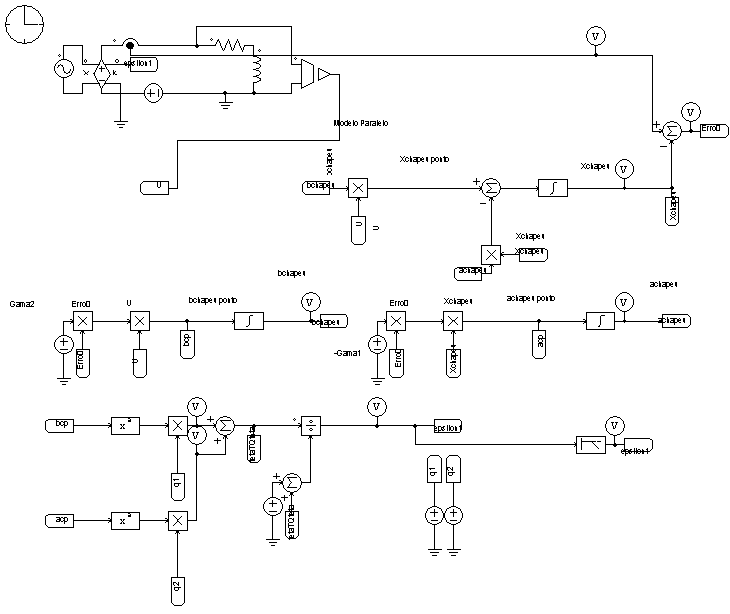
\includegraphics[width = 14 cm, height = 8 cm]{./pic/BonusMontagem.png}

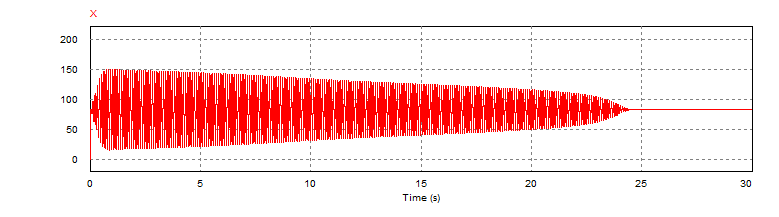
\includegraphics[width = 14 cm, height = 8 cm]{./pic/BonusX.png}

\includegraphics[width = 14 cm, height = 8 cm]{./pic/BonusXchapeu.png}

\includegraphics[width = 14 cm, height = 8 cm]{./pic/BonusEpsilon1.png}

Aqui podemos notar o comportamento de Epsilon1 como sendo um sinal que varia abruptamente, já que os valores da atualização dos parâmetros não são constantes é natural que isto aconteça. Portanto para evitar introduzir estas variações abruptas na planta escolhemos filtrar o sinal através de um filtro passa baixa de segunda ordem com frequência de corte $f_c = 1Hz$.

\includegraphics[width = 14 cm, height = 8 cm]{./pic/BonusEpsilon1Filtered.png}

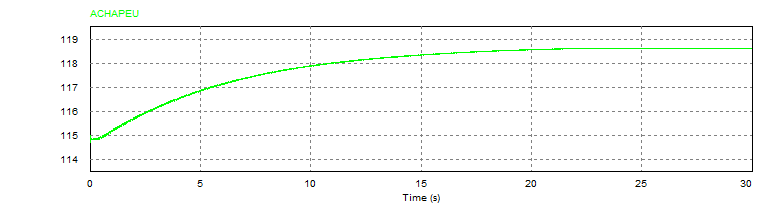
\includegraphics[width = 14 cm, height = 8 cm]{./pic/BonusTeta1.png}

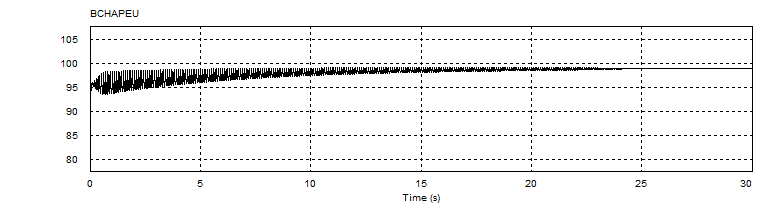
\includegraphics[width = 14 cm, height = 8 cm]{./pic/BonusTeta2.png}

E vemos que o sinal P.E desliga após os valores dos parâmetros se aproximarem suficientemente dos corretos.

\includegraphics[width = 14 cm, height = 8 cm]{./pic/BonusEsaida.png}

E também que a introdução deste método de atenuação do sinal P.E não afetou a convergência da saída do modelo para a saída da planta.



\end{document}         